\chapter{Introduzione MediaPipe}

L'applicazione sfrutta le potenzialità offerte dalla libreria \texttt{MediaPipe}, che utilizza soluzioni basate su Machine Learning nel contesto dello streaming multimediale. 
In particolare, noi abbiamo sfruttato la soluzione per il riconoscimento del movimento delle mani: \textbf{MediaPipe Hands}.\\
\\
\noindent Il nostro scopo è stato quello di interpretare ed associare movimenti delle mani a determinate gesture in modo tale da poter gestire la lettura di un documento testuale, come un pdf.\\Le funzionalità che abbiamo scelto di implementare sono:
\begin{itemize}
    \item zoom
    \item scorrimento verticale e laterale delle pagine
    \item screenshot
\end{itemize}
\noindent Abbiamo deciso di realizzare l'applicazione per ambiente Android, tramite l'utilizzo di Java ed Android Studio.


\section{MediaPipe Hands}

MediaPipe Hands offre funzionalità per il tracciamento delle mani e delle dita, utilizzando il ML per individuare 21 punti di riferimento a 3 dimensioni di una mano da un solo fotogramma.\\
Viene sfruttata una pipeline composta da due modelli che lavorano insieme:
\begin{enumerate}
    \item un modello per il \textbf{rilevamento del palmo} che opera sull'immagine completa e restituisce un riquadro di delimitazione orientato (\textit{ritaglio}) della mano. 
    \item un modello che opera sulla regione dell'immagine ritagliata definita dal modello precedente e restituisce i \textbf{punti di riferimento della mano} a 3 dimensioni.
\end{enumerate}

\noindent Il fatto di fornire al modello per i punti di riferimento un'immagine della mano accuratamente ritagliata diminuisce di gran lunga le elaborazioni necessarie, aumentando l'efficienza.\\
Inoltre, nella pipeline i \textit{ritagli} della mano possono essere generati anche in base ai punti di riferimento identificati nel frame precedente, e solo quando il modello del punto di riferimento non è più in grado di identificare la presenza della mano viene invocato il modello di rilevamento del palmo.

\subsubsection{Specifica delle pipeline}
La pipeline è implementata come un \textbf{grafo} che utilizza un \textbf{sottografo per il tracking dei punti} dal modulo \texttt{landmark} e renderizza usando un sottografo dedicato al rendering.\\Il sottografo per il tracking dei punti utilizza al suo interno un'altro sottografo per il tracking e un \textbf{sottografo per il rilevamento della mano} dal modulo \texttt{palm detection}.

\subsection{Modelli}

\subsubsection{Palm Detection Model} 

Per la rilevazione delle posizione iniziali delle mani, viene adottato un modello di rilevamento \textit{single-shot} ottimizzato per l'utilizzo in tempo reale.\\
La rilevazione delle mani è però un compito complesso per via della loro \underline{omogeneità} \underline{visiva}, a differenza per esempio del viso, che invece ha dei pattern a più alto contrasto come nelle zone degli occhi e della bocca.
Viene utilizzato perciò un \underline{contesto aggiuntivo}, come possono essere la posizione del braccio o del corpo di una persona, in modo tale da poter individuare la mano più facilmente, aumentando l'efficienza.\\
\\
\noindent Il primo componente utilizzato è un \textbf{rilevatore del palmo}, piuttosto che della mano, in quanto \textit{ritagli} di oggetti rigidi come palmi e pugni sono nettamente più semplici rispetto a quelli delle dita.\\
In secondo luogo, viene utilizzato un de/codificatore per l'estrazione di caratteristiche dall'immagine in modo da avere una maggiore consapevolezza del contesto della scena, anche per piccoli oggetti.\\
Infine, la perdita focale viene ridotta al minimo durante l'allenamento per supportare una grande quantità di ancoraggi derivanti dalla varianza su scala elevata.\\
\\
\noindent Viene stimata una precisione di circa il 96\% nella rilevazione del palmo.

\subsubsection{Hand Landmark Model} 

Dopo il rilevamento del palmo, questo modello esegue, all'interno delle regioni rilevate, la localizzazione precisa di 21 punti della mano tramite \textbf{regressione}, ovvero la previsione diretta delle coordinate.\\
Il modello apprende quindi una rappresentazione della posizione del'interno della mano coerente ed è robusto anche a mani parzialmente visibili.\\
\\
\noindent Per arrivare a questo risultato sono state annotate manualmente circa 30 mila immagini dal mondo reale con 21 coordinate 3D (valore Z preso tramite mappa di profondità). E' stato inoltre utilizzato un modello di mano sintetica su vari sfondi, mappato alle corrispondenti coordinate, in modo tale da avere un accuratezza maggiore.
\begin{figure}[H]
    \centering
    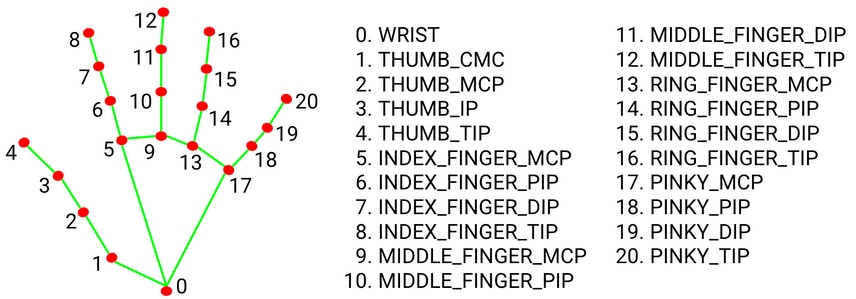
\includegraphics[width=0.8\textwidth]{images/landmarks.png}
\end{figure}


\subsection{API} 

\subsection{Opzioni di configurazione}


\paragraph{\texttt{STATIC\_IMAGE\_MODE}} Se settata a \texttt{false} (default), le immagini in ingresso vengono trattate come un flusso video, cercando di rilevare le mani nelle prime immagini di input e localizzando poi i punti di riferimento della mano. Nelle immagini successive, una volta che tutte le mani \texttt{MAX\_NUM\_HANDS} vengono rilevate e i corrispondenti punti di riferimento della mano sono localizzati, si limita a tracciare quei punti di riferimento senza invocare un altro rilevamento fino a quando non perde traccia di una qualsiasi delle mani. Questo \underline{riduce la latenza} ed è ideale per l'elaborazione di fotogrammi video.\\
Se impostato a \texttt{true}, il rilevamento manuale viene eseguito su ogni immagine di input, ideale per elaborare un batch di immagini statiche, magari non correlate.

\paragraph{\texttt{MAX\_NUM\_HANDS}} Massimo numero di mani da rilevare ($2$ a default).

\paragraph{\texttt{MODEL\_COMPLEXITY}} Complessità del modello di landmark: $0$ o $1$ (default). La precisione del punto di riferimante e la latenza aumentano con la complessità.

\paragraph{\texttt{MIN\_DETECTION\_CONFIDENCE}} Valore minimo di fiducia $[0.0, 1.0]$ nei confronti del modello di rilevamento della mano per considerare il rilevamento della mano corretto. A defult è $0.5$.

\paragraph{\texttt{MIN\_TRACKING\_CONFIDENCE}} Valore minimo di fiducia $[0.0, 1.0]$ nei confronti del modello di tracking per considerare il rilevamento dei punti di riferimento corretto. Altrimenti, il modello di rilevamento della mano (palmo) verrà richiamato all'immagine in input successiva. Di conseguenza, aumentando questo valore avremo una robustezza maggiore, a discapito di un aumento di latenza. A defult è $0.5$.

\vspace{+15 px}

\subsubsection{Output}

\paragraph{\texttt{MULTI\_HAND\_LANDMARKS}} Raccolta di mani rilevate/tracciate, ognuna rappresentata come una lista di 21 punti di riferimento a 3 dimensioni. In ogni punto \texttt{x} e \texttt{y} sono normalizzati ($[0.0, 1.0]$) rispetto alla larghezza e all'altezza dell'immagine. La coordinata \texttt{z} rappresenta invece la profondità del punto rispetto a quella del polso (considerato l'origine). Minore è il valore della \texttt{z}, più il punto è considerato vicino alla fotocamera.

\paragraph{\texttt{MULTI\_HAND\_WORLD\_LANDMARKS}} Come il precedente, ma i punti sono valutati come coordinate 3D reali in metri, con l'origine al centro geometrico approssimativo della mano.

\paragraph{\texttt{MULTI\_HAND\_HANDEDNESS}} Raccolta delle \textit{handedness} della mani (destra/sinistra). Ogni mano è composta da un'etichetta (\texttt{label}) e da un punteggio (\texttt{score}). L'etichetta è una stringa di valore \texttt{left} o \texttt{right}, mentre il punteggio rappresenta la stima della probabilità di predizione corretta della mano (sempre $\ge 0.5$, mentre l'\textit{handedness} opposta è $1-$\texttt{score}). L'\textit{handedness} viene valutata considerando che l'immagine in input è specchiata. 

\vspace{+10 px}

\subsubsection{OpenGL ES}
Per il rendering dell'input e dell'output viene utilizzato \texttt{OpenGL ES}, un sottoinsieme delle librerie grafiche di \texttt{OpenGL} pensato per dispositivi embedded.\\
Nella porzione di codice sottostante viene mostrato un esempio di utilizzo.


\begin{minted}[bgcolor=lightgray,framesep=2mm,baselinestretch=1.2,fontsize=\footnotesize,escapeinside=||,mathescape=true]{Java}
    // Vengono prima settate le opzioni di configrazione citate precedentemente
    HandsOptions handsOptions =
        HandsOptions.builder()
            .setStaticImageMode(false)
            .setMaxNumHands(2)
            .setRunOnGpu(true).build();
    Hands hands = new Hands(this, handsOptions);
    hands.setErrorListener(
        (message, e) -> Log.e(TAG, "MediaPipe Hands error:" + message));

    // Inizializzato una nuova istanza di CameraInput
    // e connessione alla soluzione MediaPipe Hands
    CameraInput cameraInput = new CameraInput(this);
    cameraInput.setNewFrameListener(
        textureFrame -> hands.send(textureFrame));

    // Inizializzato una istanza di GlSurfaceView tramite 
    // ResultGlRenderer<HandsResult> che fornisce un interfaccia 
    // per eseguire codice di rendering OpenGL definito dall'utente
    SolutionGlSurfaceView<HandsResult> glSurfaceView =
        new SolutionGlSurfaceView<>(
            this, hands.getGlContext(), hands.getGlMajorVersion());
    glSurfaceView.setSolutionResultRenderer(new HandsResultGlRenderer());
    glSurfaceView.setRenderInputImage(true);

    hands.setResultListener(
        handsResult -> {
        if (result.multiHandLandmarks().isEmpty()) {
            return;
        }
        NormalizedLandmark wristLandmark =
            handsResult.multiHandLandmarks().get(0).getLandmarkList()
                .get(HandLandmark.WRIST);
        Log.i(
            TAG,
            String.format(
                "MediaPipe Hand wrist normalized coordinates 
                (value range: [0, 1]): x=%f, y=%f",
                wristLandmark.getX(), wristLandmark.getY()));
        // Richiesta di rendering a OpenGL
        glSurfaceView.setRenderData(handsResult);
        glSurfaceView.requestRender();
        });

    // Avvio della fotocamera dopo che GLSurfaceView si è connesso
    glSurfaceView.post(
        () -> cameraInput.start(
                this,
                hands.getGlContext(),
                CameraInput.CameraFacing.FRONT,
                glSurfaceView.getWidth(),
                glSurfaceView.getHeight()));
\end{minted}
